\chapter{Character Data for the Web}\label{chap:web}

In this chapter we examine the intersection of Java character encoding 
and web technologies by showing the processing steps involved 
in sending character data via HTTP between Java programs.

The example programs for this chapter are in the code directory:
%
\displ{\filepath{src/chars/src/com/lingpipe/book/http}}
%

\section{The HTTP Protocol}\label{section:http}

How is character data sent via HTTP?
This is a misleading question.
Character data isn't sent via HTTP; \emph{bytes} are sent via HTTP.
It is up to the client and server programs to map these bytes to characters.
As we stated in \refsec{char-probs},
data sent and received across a socket is a stream of bytes.
Without knowing the character set and encoding scheme used to generate
these bytes, we cannot reliably interpret the data.

The HTTP protocol is used to send data between web servers and clients.
Web browers are but one kind of client.
Data can be sent between many web services.
Data interchange formats developed for data feeds include XML formats such as
RSS, ATOM, as well as JSON, the Javascript Object Notation.

An HTTP message consists of a header and an optional message body.
HTTP/1.1 is version of protocol in common use today.

The header consists of a series of fields.
A field is a key-value pair in clear text format separated by a colon character
and terminated by a carriage-return line-feed (CR-LF).
A field may have multiple values, in which case the values are separated by spaces,
therefore a value may not contain spaces.
The key must be ASCII text.
Non-ASCII values are allowed provided they are encoded.%
%
\footnote{See Internet Engineering Task Force (IETF) RFC 5987 for details.}
%
The header is terminated by a blank field, that is, two consecutive CR-LF sequences.
The message body, if any, follows the header.

The header fields of interest are the \code{Content-Length} and \code{Content-Type} fields.
The \code{Content-Length} field specifies the number of bytes in the body.
The \code{Content-Type} header consists of a MIME type optionally followed by 
a semi-colon followed by parameters of the form \code{attribute=value}.
The following example is taken from the HTTP/1.1 specification.
\begin{verbatim}
Content-Type: text/html; charset=ISO-8859-4
\end{verbatim}
This example specifies that message body is HTML encoded using
ISO-8859-4, the Latin-4 encoding set.
The HTTP/1.1 protocol specifies that if the \code{Content-Type} is missing from the header,
the default MIME type is text/plain and the default
character encoding is ISO-8859-1, Latin-1 (see \refsec{latin1}).

The \code{java.net} package contains classes used to implement networking applications.
We start by using \code{java.net.URL} and \code{java.net.URLConnection} objects
to send and recieve HTTP requests and responses via the example class \code{EchoHttpHeader}.
%
\displ{\filepath{src/webchars/src/com/lingpipe/book/webchars/EchoHttpHeader.java}}
%
\codeblock{EchoHttpHeader.1}
%
First we create a URL object from the first command-line argument.
If the argument doesn't start with a known protocal such as
\code{http}, \code{ftp}, \code{file}, \code{jar}, or if it is null,
the constructor will throw a \code{MalformedURLException}.
Next we create an \code{URLConnection} by calling the \code{openConnection()}
method on the \code{URL} object.
Despite its name, this method doesn't connect to the specified website, it just
creates a URLConnection object, to which setup parameters and and general 
request properties can be modified and added.
When the \code{connect()} method is invoked, the request is sent and the remote object
becomes available.  
%
\codeblock{EchoHttpHeader.2}
%
The method \code{getHeaderFields} parses the HTTP header into a map of
field names to values.
The first line of the HTTP header is the Status-Line which gives the
HTTP-version, status-code, and  reason-phrase, e.g.
\code{HTTP/1.1 200 OK}.
When we run this program with the wikipedia home page as the URL,
it returns the following headers
%
\commandlinefollow{ant -Durl="http://www.wikipedia.org" http-headers}
\begin{verbatim}  
field name: null	value: HTTP/1.0 200 OK 
field name: Age	value: 30
field name: Content-Length	value: 46388
field name: Last-Modified	value: Fri, 21 Dec ...
field name: X-Cache-Lookup	values : HIT from ...
field name: Connection	value: keep-alive
field name: Server	value: Apache
field name: X-Cache	values : HIT from cp1017.eqia...
field name: Cache-Control	value: s-maxage=3600, ...
field name: X-Content-Type-Options	value: nosniff
field name: Date	value: Tue, 15 Jan 2013 21:13:43 GMT
field name: Vary	value: Accept-Encoding
field name: Content-Type	value: text/html; charset=utf-8
\end{verbatim}
%
This page is the universal wikipedia page which consists of links to all
the language specific-wikipedias.

Next we request the Japanese wikipedia hompage
%
\commandlinefollow{ant -Durl="http://ja.wikipedia.org" http-headers}
\begin{verbatim}
field name: null	value: HTTP/1.0 200 OK 
field name: Age	value: 139
field name: Content-Language	value: ja
field name: Content-Length	value: 86186
field name: Last-Modified	value: Tue, 15 Jan 2013 ...
field name: Connection	value: keep-alive
field name: X-Cache-Lookup	values : MISS from cp1003.eqia...
field name: X-Cache	values : MISS from cp1003.eqiad.wmnet, ...
field name: Server	value: Apache
field name: X-Content-Type-Options	value: nosniff
field name: Cache-Control	value: private, s-maxage=0, ...
field name: Date	value: Tue, 15 Jan 2013 21:13:05 GMT
field name: Vary	value: Accept-Encoding,Cookie
field name: Content-Type	value: text/html; charset=UTF-8
\end{verbatim}
%
The field \code{Content-Language} is specified for the Japanese home page
but not for the universal Wikipedia page.  The contents of these pages are different
and this is reflected in the different values for the \code{Content-Length} field.
Both pages have the same Content-Type value: \code{text/html; charset=UTF-8}.
Using a Unicode charset means that almost all widely used characters in most of the
worlds languages can be used.
On my browser, most of the wikipedia languages display in thier proper font, excepting
Dhivehi, Gutisk, and a few others.

We use the header information to process the message body.
The example class \code{EchoHttpBody} retrieve the bytes from the message body and
uses the \code{charset} parameter in the \code{Content-Type} field to convert them
to characters.  
%
\displ{\filepath{src/webchars/src/com/lingpipe/book/webchars/EchoHttpBody.java}}
%
This program reads in the URL from the command line and creates a \code{URLConnection},
as in the previous example.  Next it looks for the \code{Content-Type} field and
parses out the charset name.
%
\codeblock{EchoHttpBody.2}
%
The convenience method \code{URLConnection.getContentType()} returns the entire contents
of the \code{Content-Type} field.
We use a simple regex to extract the value of the charset parameter.
If no header field is present or the charset parameter is not specified
then the encoding defaults to Latin-1.
%
\codeblock{EchoHttpBody.3}
%
Next we read in the bytes from the body and convert them to a string
using the specified charset to correctly map bytes to characters.
%
\codeblock{EchoHttpBody.4}
%
In order to write this string to the terminal we need to use a \code{java.io.Writer}
that has the same character encoding as that of the string.
We construct one using Java's \code{Standard.out}, which is a \code{PrintStream}
that writes to the standard output stream.
The resulting \code{PrintWriter} will print the characters correctly,
provided that Ant and the terminal display are correctly configured (see \refsec{ant-console-config-utf8}).

To demonstrate, we use this program to fetch the French Wikipedia home page.
\commandlinefollow{ant -Durl="http://fr.wikipedia.org" http-body}
\begin{verbatim}   
URL: http://fr.wikipedia.org
Content-Type: text/html; charset=UTF-8
charset: UTF-8
HTTP Response body:
<!DOCTYPE html>
<html lang="fr" dir="ltr" class="client-nojs">
<head>
<title>Wikipédia, l'encyclopédie libre</title>
<meta charset="UTF-8" />
<meta name="generator" content="MediaWiki 1.21wmf6" />
\end{verbatim}
The first four lines of output are diagnostics printed by the \code{EchoHttpBody} program itself.
The remaining lines are the beginning of the French Wikipedia homepage,
which is an HTML document.


\section{MIME Types and the  \code{charset} Parameter}

MIME types are specified as type/subtype pairs optionally, followed by a parameter. 
MIME type \code{text/*} allows the \code{charset} parameter and includes type/subtypes:
\begin{verbatim} 
text/plain 
text/html
text/xml
\end{verbatim}
The MIME-type standard (see \url{http://www.ietf.org/rfc/rfc2046.txt}) specifies
that the default \code{charset} parameter for type \code{text} is ASCII (see \refsec{ascii}).

The type \code{text/xml} is a legacy type; for XML data the type 
\code{application/xml} is preferred. 
Data in a defined dialect of XML is specified accordingly.
For example, RSS feed data should be of type \code{application/rss+xml}.
Examples of MIME-types for XML and dialects of XML include:
\begin{verbatim}  
application/xml
application/rss+xml 
application/xhtml+xml 
\end{verbatim}  
The \code{application/xml} and \code{+xml} MIME types can take an
optional charset parameter.  If none is present it is up to the application
to infer or guess the character encoding used based on rules laid out
in the XML 1.0 Recommendation.  See \url{http://www.w3.org/TR/REC-xml/#sec-guessing}.

\subsection{MIME Type \code{application/x-www-form-urlencoded}}\label{section:urlencoding}

The MIME type \code{application/x-www-form-urlencoded}
is so named because it is the default encoding used by the browser
to send a POST request from a web form element.
This encoding allows URLs that contain non-ASCII characters to be sent via an HTTP request.

A URL encoded string contains only alphanumeric ASCII characters plus the characters
hyphen, underscore, period, and asterisk. 
The percent character is allowed 
but is interpreted as the start of a special escaped sequence.
To encode a string, spaces are converted to '+' and
all other characters are converted by taking their byte value
(the UTF-8 character encoding is recommended)
and converting each byte to the sequence \emph{\%xy} where \emph{xy} correspond to the
two-digit hex value of the 8 bits.
Because the percent character is meaningful,
if it occurs in the data it will be URL encoded as \code{\%25}.

The \code{Java.net} package contains two convenience classes, \code{URLEncoder}
and \code{URLDecoder} which provide static methods to encode and decode strings.
The example class \code{EncodeDecodeUrl} encodes and decodes string.
%
\displ{\filepath{src/webchars/src/com/lingpipe/book/webchars/EncodeDecodeUrl.java}}
%
\codeblock{EncodeDecodeUrl.1}
%
We construct the string literal \emph{\'{A} votre sant\'{e}} using the hexadecimal
representation of the Unicode code points for the non-ASCII characters.
We use the static method \code{URLEncoder.encode} to create a URL-encoded version
and then decode that.  Finally we print out all three strings, using a
\code{PrintWriter} whose character encoding is UTF-8.
%
\commandlinefollow{ant url-encode}
\begin{verbatim}  
string: À votre santé!
url encoded: %C3%80+votre+sant%C3%A9%21
decoded: À votre santé!
\end{verbatim}


\section{XML}

In this section we focus on processing text data in XML documents.
There are many good books XML processing.
We particularly recommend \emph{Java and XML} by McLaughlin et.al.
published by O'Reilly.

\subsection{XML Character Encoding}

The character encoding used for the XML document is of primary importance.
It is specified in the opening XML declaration, e.g.
\begin{verbatim} 
<?xml version="1.0" encoding="UTF-8" ?>
\end{verbatim}  
The encoding declaration is optional.
The default character encoding is UTF-8.

XML was designed for Unicode data.
Even if the document's declared encoding is a 
legacy encoding such as Latin-1 (ISO-8859-1),
the document can contain any legal Unicode character.
Characters outside of the declared encoding can be represented 
via that characters numerical character refernce (NCR), see below.

When XML is sent as the body of an HTTP message, the HTTP \code{Content-Type} 
header should match the declared encoding.  If the HTTP \code{Content-Type} header
is unspecified, the message body encoding defaults to Latin-1.
If the body is decoded using the wrong charset then either the message may be
corrupted or an exception may be thrown.


\subsubsection{Allowed Characters}

As we saw in \refsec{unicode}, not all Unicode characters are legal XML characters.
ASCII control characters are not legal Unicode, excepting tab, carriage return, and linefeed.
XML also disallows some Unicode characters in the surrogate code blocks.
XML documents which have been created from non-UTF data, such as legacy data
encoded in Latin-1 (ISO-8859-1) or Windows-1252, 
may sometimes contain characters that fall outside of the allowed values.
This is likely to cause a parser error, especially if the legacy character encoding
is not declared in the opening XML declaration.


\subsubsection{Characters and Entity References}\label{section:xml-entity-refs}

XML entity references are be used in place of characters, either as a way of
escaping reserved characters that would otherwise be interpreted as markup,
or when the character symbol is not available.
The XML syntax markers cannot be used as regular characters in text; 
use the following set of predefined entities instead:
\code{\&lt;} for < (open tag), \code{\&gt;} for > (close tag), \code{\&amp;} for \&,
\code{\&apos;} for ' (single quote), and \code{\&quot} for " (double quote).

Many other characters have named entity references.  The full list of 
entity definitions for characters is maintained by the W3C and is available here
\urldisplay{http://www.w3.org/TR/xml-entity-names/}.

All permitted Unicode characters may be represented with a numeric character reference.
The numerical character reference is the value of the Unicode code point
expressed in either in decimal or hex, 
prefixed by ampersand and followed by a semicolon.
Decimal values start with \# (hashcode), hexidecimal values start with \#x.
For example, the Greek capital letter Sigma has Unicode code point U+03A3
(hex value 3A3, decimal value 931).  In XML (and HTML) this is written as either
\code{\&\#931;}, \code{\&\#0931;}, \code{\&\#3A3;},  or \code{\&\#03A3;}.

\subsubsection{Parsed and Unparsed Character Data}\label{xml-pcdata-cdata}

An XML document must contain a single top-level element.
Within this element, text is either character data or markup.
The markup consists of the angle brackets (<>) and the names inside them.
All text that is not markup is character data.

By default, XML processors parse all text in an XML document
in order to find markup and entity references.
CDATA is unparsed character data within an XML element.
A CDATA section starts with \code{<!CDATA[} and ends with \code{]]>}.
Nested CDATA sections are not allowed.  The sequence \code{]]>}
Is always interpreted as the close of a CDATA section.
If this sequence occurs in the text itself, it must be placed outside
of the CDATA section and if more text follows, then a new CDATA section is opened.

CDATA sections may be useful in situations where the contents of
an element contain many instances of the XML syntax markers, for example, when the
contents are a Javascript or HTML fragments.  In a CDATA sections, these characters can
be used directly, instead of using entity references.  However, because the CDATA
contents are unparsed, no entity references can be used.  Thus the contents of the
CDATA section are restricted to only the legal XML characters in the declared encoding.


\subsection{DOM and SAX APIs for XML}\label{xml-dom-sax}

An XML document consists of a single top-level element which contains
nested XML elements.   There are two approaches to processing XML:
DOM and SAX.

The DOM (Document Object Model) approach to XML maps the XML document into a tree structure
and then navigates that tree.  
Once fully constructed, any part of the tree can be accessed and the structure of 
the tree itself can be modified.
The DOM tree for large documents will require large amounts of memory.

SAX, the Simple API for Java, is an event-based sequential access
parser API.  It is a streaming interface.  Applications using SAX
receive event notifications about the XML document being processed as each
element and attribute are encountered in sequential order starting at the
top of the document, and ending with the closing of the ROOT
element. The application must implement handlers to deal with the different events.
SAX parsers can process XML in
linear time and is memory efficient.

Here is the ``Hello World'' XML document
\begin{verbatim}
<?xml version="1.0"?>
<!DOCTYPE foo SYSTEM "foo.dtd">
<foo><bar>Hello, world!</bar></foo>
\end{verbatim}

An event-based parser treats this as a series of linear events
that are reported to the calling application as
\begin{verbatim}
start document
start element: foo
start element: bar
characters: "Hello, world!"
end element: bar
end element: foo
end document
\end{verbatim}

\subsection{SAX Example: Trace Events and Get Characters}

The example class \code{TraceSaxEvents} illustrates 
how the SAX parser/handler pattern works.
It uses the parsers and handlers in the
\code{org.xml.sax} package to report on parsing events and it
echos all characters found in the elements in that document.
%
\displ{\filepath{src/webchars/src/com/lingpipe/book/webchars/TraceSaxEvents.java}}
% 
First we create a class \code{TraceHandler}.
%
\codeblock{TraceSaxEvents.1}
%
The class \code{org.sax.xml.helpers.DefaultHandler} provides default implementations
for the callback methods in the core SAX2 handler classes.
The \code{TraceHandler} class overrides the methods 
\code{startDocument, endDocument, startElement, endElement, characters}
so that these events are reported to the console.
The \code{characters} method prints the characters enclosed by
the vertical bar (|) character.
%
\codeblock{TraceSaxEvents.2}
%
We use the \code{XMLReaderFactory} to get an \code{XMLReader}.
We set the XMLReader's content handler to an new instance
of \code{TraceHandler}.
The XMLReader parses the input.
The handler's callback methods are called as the parser encounters
XML markup.

Xml elements may contain text interleaved with other elements.
We have included a small example file with this chapter,
%
\displ{\filepath{src/webchars/foo.xml}}
\begin{verbatim}
<?xml version="1.0"?>
<foo> 
 tok1 
 <bar> tok2 </bar>  tok3 
 <bar> tok4 
           tok5 </bar>
</foo>
\end{verbatim} 
Here is the output from running \code{TraceSaxEvents} on this file
\begin{verbatim} 
startDocument
startElement: foo
characters: | 
 to|
characters: |k1 
 |
startElement: bar
characters: | tok2 |
endElement: bar
characters: |  tok3 
 |
startElement: bar
characters: | tok4 
           tok5 |
endElement: bar
characters: |
|
endElement: foo
endDocument
\end{verbatim}
The XMLReader parses data from the InputSource as it becomes available.
There are two consecutive callbacks to the \code{characters} method to
retrieve the initial content which includes whitespace, the string \emph{tok1},
another space plus a newline.
All character and whitespace that are outside of XML markup tags are returned
by the \code{characters} method.

\subsection{DOM Example: Encode Characters for XML}

The example class \code{JDomGenerateXml} generates an XML document
which contains text content in several languages.
The character encoding is specified by the user.
Depending on the specified encoding, different subsets of the
character data must be be escaped.
%
\displ{\filepath{src/webchars/src/com/lingpipe/book/webchars/JDomGenerateXml.java}}
%
This program uses the open-source API JDOM2 from \url{http://www.jdom.org}
to create a document and write it out to disk.
The JDOM2 jarfile is included in the subdirectory of the \code{src/webchars/lib}.
%
\codeblock{JDomGenerateXml.2}
%
We construct an XML document in a top-down fashion by first creating
the root XML element and adding it to a new XML document.
The top-level element of this document is a \code{<toast\_set>}.
It contains multiple \code{<toast>} elements which have 
an attribute named \code{lang} and whose text content consists
of a toast in the language.
%
\codeblock{JDomGenerateXml.1}
%
These toasts are specified as Java Strings using Unicode escapes 
for all non-ascii characters.
%
\codeblock{JDomGenerateXml.3}
%
We add toasts in English, French, Russian, and Korean.
%
\codeblock{JDomGenerateXml.4}
%
This program takes two command line arguments.
The first argument, \code{args[0]}, specifies the character encoding,
and the second specifies the name of the output file.
The \code{org.jdom2.output.XMLOutputter} outputs the contents of an
XML document as a stream of bytes.
A \code{org.jdom2.output.Format} object controls
the encoding used to do this conversion.
The method \code{setEncoding(String encoding)} overrides the default
encoding.
The encoding argument is also used to set the character encoding on 
the \code{OutputStreamWriter} that the \code{XMLOutputter} is writing to.
This is necessary because a \code{Writer} configuration cannot be queried
or controlled by the \code{XMLOutputter}.

\code{Format.getPrettyFormat()} returns a new Format object that
performs whitespace beautification with 2-space indents, uses the
UTF-8 encoding, doesn't expand empty elements, includes the
declaration and encoding, and uses the default entity escape strategy.
An escape strategy encapsulates the logic that determines
which characaters should be formatted as character entities.
The set of syntax markers are always formatted as character entities
(see \refsec{xml-entity-refs}).  The method \code{canEncode} in class
\code{java.nio.charset.CharsetEncoder} is used to identify characters
whose Unicode code point is not mapped into a character in the specified encoding
(see \refsec{charset-encoder}).

To see how entities are escaped under different encodings
we run \code{JDomGenerateXML} three times via the ant task \code{gen-xml}
to generate files encoded as UTF-8, ASCII, and Cyrillic.
%
\commandlinefollow{ant gen-xml -Dencoding="UTF-8" -Dfile="enc-utf8.xml"}
\commandlinefollow{ant gen-xml -Dencoding="ASCII" -Dfile="enc-ascii.xml"}
\commandline{ant gen-xml -Dencoding="KOI-8" -Dfile="enc-koi8.xml"}

\reffig{xml-escapes} shows
these three output files displayed in the emacs text editor.
Emacs has the fonts to display all characters and diacritics in
the Roman, Cyrillic, and Korean alphabets.
In the UTF-8 file, none of the characters have been escaped, because
UTF-8 contains character mappings for all Unicode code points.
In the ASCII file, all non-ASCII characters have been escaped.
The KOI-8 encoding contains characters corresponding to
the code points for ASCII and Cyrillic characters
but not \'{e} or any of the glyphs for Korean.

\begin{figure}
%\begin{center}
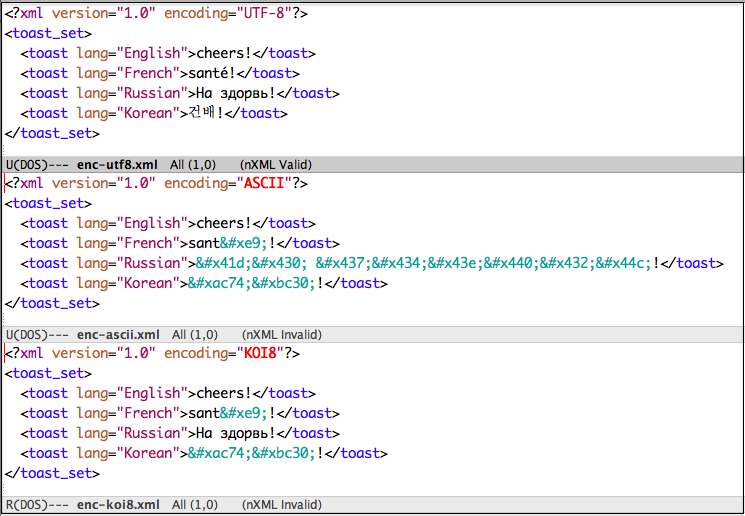
\includegraphics[width=5.0in]{pngs/xmlencodings.png}
%\end{center}%
\vspace*{-18pt}
\caption{Entity escapes for different encodings.}\label{fig:xml-escapes}
\end{figure}

\section{HTML}

HTML was designed for documents sent via HTTP from web servers
to web browsers (or other web client, collectively known as User-Agent programs).
Bytes are sent via HTTP; characters are displayed by the browser.

The browser determines the character encoding.
The browser can use the \code{charset} parameter on the
\code{Content-Type} header field of the HTTP response
from the web server or it can try to get the encoding information
from the \code{meta} tags in the \code{head} section of the HTML document
or it can try to determine the encoding heuristically
(see \refsec{encoding-detection}).
The user can always override the chosen character encoding 
via controls on the browser.

HTML meta-tags are used either to emulate the use of the HTTP response header, 
or to embed additional metadata within the HTML document.
These tags have the form \code{<meta http-equiv="foo" content="bar">}.
The tags
\begin{verbatim}
<meta http-equiv="Content-Type" content="text/html; charset=UTF-8">
<meta charset="UTF-8">
\end{verbatim}
emulate the \code{charset} parameter of the \code{Content-Type} header field.

Return to HTML example:  Hello World, Hello World Japan. 
Examine browser, override heading.

\subsection{HTML Character and Entity References}

As in XML, the characters that are syntax markers cannot be used directly
in text and the corresponding predefined entities must be used instead:
\code{\&lt;} for < (open tag), \code{\&gt;} for > (close tag), \code{\&amp;} for \&,
\code{\&apos;} for ' (single quote), and \code{\&quot} for " (double quote).

The HTML specification defines a large set of character entity references:
\urldisplay{http://www.w3.org/TR/html4/sgml/entities.html}
\urldisplay{http://www.w3.org/TR/html5/syntax.html\#named-character-references}

Numeric character references may also be used.
The numerical character reference is the value of the Unicode code point
expressed in either in decimal or hex, 
prefixed by ampersand and followed by a semicolon.
See \refsec{xml-entity-refs}.

Next to HTML example:  toast\_ncr.html - using NCR escapes always works

\subsection{Parsing HTML}

Parsing HTML documents is challenging because although standards
have been developed for HTML, they are often not met.
Therefore applications which mine HTML documents for text data
must be able to handle ill-formed HTML.
When we need to extract text data from an HTML document,
we use the NekoHTML parser.

http://nekohtml.sourceforge.net/

Example:  get character encoding from header, extract all text inside paragraph elements.
Simple example which extracts all content inside a paragraph.

\section{JSON}

MIME-type application/json

simple json

Escapes for JSON reserved characters.

\subsection{Parsing JSON}

\subsection{Generating JSON}


